\documentclass[fleqn]{jbook}
\usepackage{physpub}

\begin{document}

\begin{question}{教育 物理}{}


\begin{subquestions}
\SubQuestion
  質量$M$、半径$R$の一様な円盤が、傾斜角$\theta$の坂をすべらずに
  転がり落ちる運動を考える。斜面に沿って$x$軸をとり、重力加速度を
  $g$、ころがりまさつ力を$F$として次の問に答えよ。

  \begin{subsubquestions}
  \SubSubQuestion
    円盤重心の$x$方向の運動方程式を示せ。

  \SubSubQuestion
    円盤の回転軸まわりの慣性モーメント$I$を求め、回転に関する
    運動方程式を示せ。

  \SubSubQuestion
    $x$方向の速度$v$と、回転角速度$\omega$の関係を示せ。

  \SubSubQuestion
    以上の関係を整理して、$x$方向の加速度が、まさつがなかった場合の
    何倍になっているのかを求めよ。

  \end{subsubquestions}


\SubQuestion
  図に示すように金属線で出来た正方形のループが$yz$面内にある。
  ループの上半分に強さ$B[T]$の一様磁場がループ面と垂直($x$軸方向)
  にかかっており、また、ループは下方に重力を受けているものとする。\\
%
  ループの一辺の長さを$L[{\rm m}]$、金属線の断面積を$s[{\rm m^2}]$、
  金属の密度を$d[{\rm kg/m^3]}$、金属の抵抗率を$\rho[{\rm \Omega m}]$、
  重力加速度を$g[{\rm m/s^2}]$として、以下の問に答えよ。ただし、
  空気の抵抗は無視し、ループが回転してしまうことは無いものとする。
  また、ループは十分に大きいとして、ループ全体が磁場の外に出てしまう
  場合を考慮する必要はない。\vspace*{-4mm}

  \parbox[t]{100mm}{
  \begin{subsubquestions}
  \SubSubQuestion
    ループが速度$v$で落下しているとき、ループに流れる電流$I$の
    向きを図示し、その大きさを求めよ。

  \SubSubQuestion
    ループにながれる電流と磁場$B$とによってループが受けるローレンツ力
    $F$の方向を図示し、その大きさを求めよ。

  \SubSubQuestion
    ループの落下運動をあらわす運動方程式を書き下せ。
 
  \SubSubQuestion
    ループの初速を$0$として落下速度$v$を時間の関数として求め、\\
    $v$の変化の様子をグラフに示せ。
  \end{subsubquestions}
  }\parbox[t]{60mm}{
  \begin{center}
    \mbox{\includegraphics[clip]{1993phys-1.eps}}
  \end{center}}
  \vspace*{-6mm}

\SubQuestion
  圧力$p$と単位体積あたりの内部エネルギー$u$の間に
%
  \[p=\frac{1}{3}u \]
%
  の関係が成り立つ気体がある(光子気体)。$u=u(T)$が温度$T$のみの
  関数であるとして、その関数形を求めたい。以下の問に答えよ。

  \begin{subsubquestions}
  \SubSubQuestion
    断熱過程において圧力$p$と体積$V$の間に$pV^{4/3}=一定$の関係が
    成り立つことを示せ。

  \SubSubQuestion
    四つの状態$A,B,C,D$を通り、等温膨張$(A\rightarrow B)$、断熱膨張
    $(B\rightarrow C)$、等温圧縮$(C\rightarrow D)$、断熱圧縮
    $(D\rightarrow A)$という四つの準静的過程からなる可逆サイクルを
    考える。このサイクルの$p-V$図の概略を描け。但し、状態$A,B,C,D$に
    おける体積をそれぞれ$V_A,V_B,V_C,\\V_D$とし、等温過程
    $A\rightarrow B$及び$C\rightarrow D$における温度をそれぞれ$T_1$
    及び$T_2$とする。

  \SubSubQuestion
    上記のサイクルで、等温過程$A\rightarrow B$及び$C\rightarrow D$の
    間に吸収する熱量をそれぞれ$Q_1$及び$Q_2$とするとき、$Q_1,Q_2$を
    求めよ。

  \SubSubQuestion
    このサイクルが可逆であることを用いて
%
    \[\frac{u(T_1)^{1/4}}{T_1}=\frac{u(T_2)^{1/4}}{T_2} \]
%
    が成り立つことを示せ。

    [参考:これにより、Stefan-Boltzmann の法則 $u(T)=\sigma T^4$
    ($\sigma$は定数)が得られる。]
  \end{subsubquestions}
\end{subquestions}
\end{question}
\begin{answer}{教育 物理}{}

\begin{subanswers}
\SubAnswer
  問題の状況は右図の様である。

  \begin{subsubanswers}
  \vspace*{-5mm}\parbox[t]{85mm}{
  \SubSubAnswer
    重心の運動方程式は次の通りである。
%
    \[ M\ddot{x} = Mg\sin\theta - F \]
%


  \SubSubAnswer
    円盤の密度を $\rho = M/\pi R^{2}$として慣性モーメント $I$は
%
    \[ I = \int_{0}^{R} \rho r^{2} \cdot 2\pi r \cdot \d{r}%
         = 2\pi\rho \frac{R^{4}}{4} = \frac{1}{2}MR^{2} \]
%
    }\parbox[t]{70mm}{\vspace*{-15mm}
    \begin{center}
      \mbox{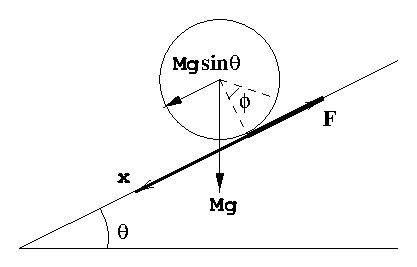
\includegraphics[clip]{1993phys-2.eps}}
    \end{center}}\\
%
    となる。回転の運動方程式は、図の反時計回りを回転角速度
    $\omega$の正の向きとして、
%
    \[ I\dot{\omega} = FR \hspace{15mm}%
       \Yueni \frac{1}{2}MR^{2} \dot{\omega} = FR \]
%

  \SubSubAnswer
    すべりがないので明らかに次式が成り立つ。
%
    \[ v = R\omega \]
%

  \SubSubAnswer
    前問での結果を総合して、摩擦力 $F$を消去すると、
%
    \[ \dot{v} = \frac{2}{3}g\sin\theta \]
%
    を得る。摩擦があるときは摩擦がないときの$\frac{2}{3}$倍の加速度
    をもつことになる。

  \end{subsubanswers}



\SubAnswer
  \begin{subsubanswers}
  \SubSubAnswer
    ループを貫く磁束を$\Phi$としたとき、起電力$V$はFaradayの電磁誘導
    の法則より、
%
    \[ V = - \Deriver{\Phi}{t} \]
%
    である。起電力の向きは磁場に対して右向きであるが、問題の図では
    ループの反時計回りである。

    磁束の変化分はループのうち$y$軸と並行な上側の金属線が通過する
    磁束である。金属線の速度 $v$が負の値であることに注意して
    $\d{\Phi} = B v L \d{t}$よって起電力は
%
    \[ V = -BvL \quad (\,>0\,) \]
%
    ループの抵抗 $R$ は $R=\rho 4L/s$と表される。流れる電流 $I$は
%
    \[ I = \frac{V}{R} = -\frac{Bsv}{4\rho} \quad (\,>0\,) \]
%
    電流は図では反時計回りに流れる。

  \SubSubAnswer
    $z$軸に平行な線にかかる力は相殺し、$z$軸に垂直な線に働く力のみが
    残る。
%
    \[ F = IBL = -\frac{B^{2}sLv}{4\rho} \]
%
    この力は上向きである。

  \SubSubAnswer
    ループの質量 $m$ は $m=4Lsd$と表される。運動方程式は
%
    \[ m\dot{v} = F - mg \]

  \SubSubAnswer
    \parbox[t]{75mm}{
    前問で得られた運動方程式を整理して
%
    \[ \dot{v} = -\frac{B^2}{16\rho d}v - g \]
%
    となる。これを初期条件$v(0)=0$のもとで解くと、
%
    \[ v = \frac{16\rho dg}{B^{2}} \left[%
             \exp{\left( -\frac{B^2}{16\rho d}t\right)} - 1%
           \right] \]
%
    この $v$の時間変化は右図の様である。
%
    }\parbox[t]{75mm}{\vspace*{-10mm}
    \begin{center}
      \mbox{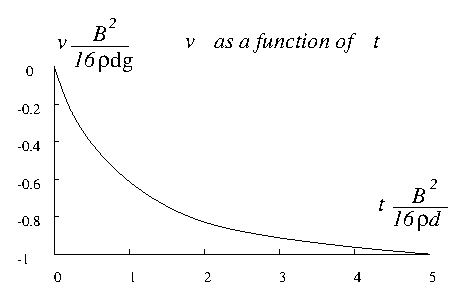
\includegraphics[clip]{1993phys-3.eps}}
    \end{center}}

  \end{subsubanswers}


\SubAnswer
  \begin{subsubanswers}
  \SubSubAnswer
    全内部エネルギー$U$は
%
    \[ U=u(T) \times V = 3pV  \hspace{15mm}%
       \Yueni \d{U}=3(p\d{V}+V\d{p}) \]
%
    断熱過程であるので
%
    \[ \d{U}=\d{Q}'-p\d{V}=-p\d{V} \]
%
    よって、
%
    \[ 4p\d{V}+3V\d{p}=0%
       \hspace{3mm} \rightarrow \hspace{3mm}%
       \frac{4}{3}\frac{\d{V}}{V}=-\frac{\d{p}}{p}%
       \hspace{3mm} \rightarrow \hspace{3mm}%
       \frac{4}{3}\log{V}=-\log{p}+c \]
    \[ \Yueni pV^{4/3}= {\rm const} \] 

  \parbox[t]{75mm}{
  \SubSubAnswer
    等温過程で$u(T)$は一定なので$p$も一定となる。\\
    $p-V$図は右図の通り。

  \SubSubAnswer
    等温過程では$p$が一定 $\d{p}=0$ なので
%
    \[ \d{U}=3p\d{V} \]
%
    となる。また流入する微小熱量を $\d{Q}'$ として
%
    \[ \d{U}=\d{Q}'-p\d{V} \]
%
    よって
%
    \[ \d{Q}'=4p\d{V} \]
%
    }\parbox[t]{80mm}{
    \begin{center}
      \mbox{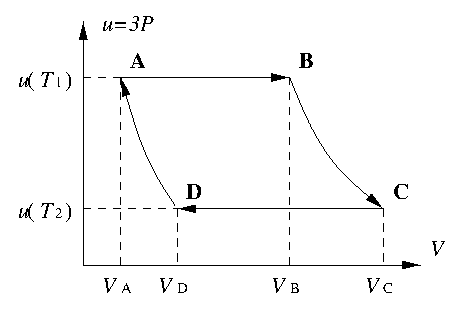
\includegraphics[clip]{1993phys-4.eps}}
    \end{center}}\\
%
    これより流入する熱量は体積の差に比例することがわかる。熱量
    $Q_1,Q_2$ は以下の通り。
%
    \begin{eqnarray*}
      Q_1 &=& \int^{\rm B}_{\rm A}\d{Q}' = 4p(V_{\rm B} - V{\rm _A})%
           =  \frac{4}{3}u(T_1)(V_{\rm B}-V_{\rm A}) \quad >0 \quad 吸熱 \\
      Q_2 &=& \frac{4}{3}u(T_2)(V_{\rm D}-V_{\rm C}) \quad <0 \quad 廃熱
    \end{eqnarray*}

  \SubSubAnswer
    可逆なのでエントロピー収支は$0$である。すなわち、
%
    \[ \frac{Q_1}{T_1}+\frac{Q_2}{T_2}=0 \]
%
    前問の結果を代入して
%
    \[ \frac{4}{3}\frac{u(T_1)(V_{\rm B}-V_{\rm A})}{T_1}%
      +\frac{4}{3}\frac{u(T_2)(V_{\rm D}-V_{\rm C})}{T_2} =0 \]
%
    設問(i)で示された定理から
%
    \[ u(T_1)V_{\rm A}^{4/3} = u(T_2)V_{\rm D}^{4/3} \hspace{10mm}%
       u(T_1)V_{\rm B}^{4/3} = u(T_2)V_{\rm C}^{4/3} \]
%   
    が得られ、これから$V_{\rm C},V_{\rm D}$を$V_{\rm A},V_{\rm B}$で
    表わしたものを代入すると
%
    \[ \frac{u(T_1)}{T_1}%
      -\frac{u(T_2)}{T_2} \left(%
         \frac{u(T_1)}{u(T_2)}%
       \right) ^{3/4} = 0 \]
%
    となり、これにより
%
    \[ \frac{u(T_1)^{1/4}}{T_1}=\frac{u(T_2)^{1/4}}{T_2} \]
%
    が示される。

  \end{subsubanswers}
\end{subanswers}
\end{answer}


\end{document}
